In today's age of big data, machine learning and various other fields, it's important to have ways to quickly analyse these datasets and ideally find patterns within. Non-negative matrix factorization is one of the paradigms suitable for that task.

In layman's terms, what NMF does is that when we are given a large set of data, for example a matrix representing books and their review scores from people, we can extract certain hidden "features" from it using NMF, in this case representing e.g. various genres (basis matrix) and how prominent they are in a given book (weight matrix). And then, using these two matrices, we are able to estimate or even predict what kind of books a user would like - this is a simple example of a possible recommendation algorithm.

\section{Linear dimensionality reduction}
Non-negative matrix factorization, or NMF, falls under \emph{linear dimensionality reduction} techniques. These are used widely for noise filtering, feature selection or compression, among others.

LDR can be defined as following: \cite{nmf_why_how}

\begin{align}
x_j &\approx \sum_{k=1}^{r}w_kh_j(k) &\text{for some weights $h_j \in \mathbf{R}^r$}
\end{align}

where given a data set of size $n$, we define $x_j \in \mathbf{R}^p$ for $1 \leq j \leq n$, $r < \min(p,n)$, and $w_k \in \mathbf{R}^p$ for $1 \leq k \leq r$.

What this effectively means is that we represent $p$-dimensional data points in a $r$-dimensional linear subspace, with basis elements $w_k$ and data coordinates given by vectors $h_j$. LDR defined in this manner is equivalent to low-rank matrix approximation, which is the essence of non-negative matrix factorization.

\section{NMF definition}
Non-negative matrix factorization solves the following NP-hard problem:

Given a non-negative matrix $V$, find non-negative matrix factors $W$ and $H$ such that:

\begin{align}
V \approx WH
\end{align}

That is, given a set of multivariate $n$-dimensional data vectors, we place these vectors in the columns of a $n \times m$ matrix $V$, where $m$ is the amount of examples we have. We then approximately factorize this matrix into two different matrices: a $n \times r$ matrix $W$ and a $r \times m$ matrix $H$. We generally choose $r < \min(n,m)$ (though this is not required) so that the two matrices are smaller than the original matrix $V$, essentially compressing it. \cite{nmf_algorithms}

\section{Classification}
NMF is as of currently still a relevant research topic, and has been explored by researchers from many different fields including mathematicians, statisticians, computer scientists or biologists. Given the wide range of use, over time it lead to different variations and additional constraints on the algorithms. Therefore, a taxonomy system was proposed in \cite{wang_zhang_2013}, outlined below.

\begin{figure}[ht]
	\caption[NMF classification]{The NMF classification as per \cite{wang_zhang_2013}.}
	\centering
	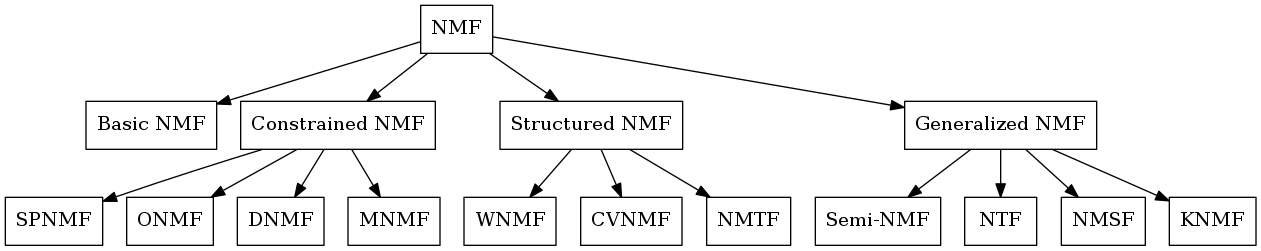
\includegraphics[width=\textwidth]{nmf_classification.png}
\end{figure}

\subsection{Basic NMF}
This is the basic model which only enforces non-negativity, and which all the following ones build upon.

However, due to its unconstrained nature, without any other constraints there are many possible solutions  which may lead to the algorithm's performance to vary. Further constraints outlined below help in the search of unique solutions and optimizing for specific scenarios.

\subsection{Constrained NMF (CNMF)}
Constrained NMF imposes additional constraints on the resulting matrices, namely:

\begin{description}
	\item[Sparse NMF] SPNMF, sparseness constraint
	\item[Orthogonal NMF] ONMF, orthogonality constraint
	\item[Discriminant NMF] DNMF, couples discriminant information along with the decomposition
	\item[NMF on manifold] MNMF, preserves local topological properties
\end{description}

\subsection{Structured NMF (SNMF)}
Structured NMF modifies standard factorization formulations:

\begin{description}
	\item[Weighed NMF] WNMF, attaches weights to different elements relative to their importance
	\item[Convolutive NMF] CVNMF, considers time-frequency domain factorization
	\item[Non-negative Matrix Trifactorization] NMTF, decomposes the data into three matrices
\end{description}

\subsection{Generalized NMF (GNMF)}
Generalized NMF can be considered a broader variant of Basic NMF, where conventional data types or factorization modes may be replaced with something different. It's split as follows:

\begin{description}
	\item[Semi-NMF] relaxes the non-negativity constraint on a specific factor matrix
	\item[Non-negative Tensor Factorization] NTF, generalizes the model to higher dimensional tensors
	\item[Non-negative Matrix-set Factorization] NMSF, extends the data sets from matrices to matrix-sets
	\item[Kernel NMF] KNMF, non-linear model of NMF
\end{description}

\section{Properties}
The additional constraint of non-negativity is important, as results show that it leads to a natural higher sparseness in both the basis matrix ($W$) and the encoding matrix ($H$). Additionally, non-negativity leads to a parts-based representation, which is similar to how our brains are presumed to work, basically combining parts in an additive manner to form a whole instead of subtracting. \cite{nmf_parts_objects} This sparseness makes it even easier to further compress the resulting matrices, saving us more space.

However this isn't without any downsides. While the concept of adding parts together seems to make a lot of sense, there is an issue. Since NMF employs a holistic approach, the additive parts learned by it in an unsupervised mode only considers features on a global level, and does not allow for representation of spatially localized features. \cite{li_spatial_lnmf_2001}

So while on paper NMF might seem better than PCA or SVD for a parts-based representation, it only comes at a cost of increased complexity, and since both PCA and SVD have a more compact spectrum than NMF, we must consider if this is worth the trade-off. \cite{wang_zhang_2013}

\section{Algorithms}
For the purposes of this thesis, we will only consider algorithms for Basic NMF. While NMF has been widely used in sound analysis etc. as we'll see below, its use for audio compression specifically is rare and there are limited resources to provide insight into utilizing possible constraints, therefore we will only be using the standard version.

Finding a decomposition of a matrix $V$ into matrices $W$ and $H$ is an NP-hard problem, and as such, the resulting matrices are generally only approximated over a number of iterations of an optimization algorithm. What this means in practice is that it's likely a result we'll find is sub-optimal or a local minimum.

\subsection{Cost function}
When using iterative updates, in each step of the process we need to evaluate the quality of the approximation. The function that does this is called the \emph{cost function}, or \emph{objective function}.

There are two simple commonly used functions. Firstly, we can use squared Euclidean distance: \cite{pentti_pmf_1997}

\begin{align}
||A-B||^2 = \sum_{ij}(A_{ij} - B_{ij})^2
\end{align}

This is lower bounded by 0, which it only is equal to if $A = B$.

Another metric we can use is based on Kullback-Leibler divergence, and is defined as such: \cite{nmf_algorithms}

\begin{align}
D(A||B) = \sum_{ij} \left( A_{ij} \log \frac{A_{ij}}{B_{ij}} - A_{ij} + B_{ij} \right)
\end{align}

\subsection{Update rules}
With the cost function in place, we now need a function to apply each iteration to try and minimize the value of the cost function. It has been found that a good compromise between speed and ease of implementation is to use what's called \emph{multiplicative update rules}. \cite{nmf_algorithms} Despite being over 15 years old, they are still very commonly used exactly for this reason.

For non-increasing Euclidean distance $||V - WH||$, if $W$ and $H$ are at a stationary point of distance, we may use these rules:

\begin{align}
H_{a \mu} & \leftarrow H_{a \mu} \frac{(W^TV)_{a \mu}}{(W^TWH)_{a \mu}} \\
W_{ia} & \leftarrow W_{ia} \frac{(VH^T)_{ia}}{(WHH^T)_{ia}}
\end{align}

And for non-increasing divergence $D(V||WH)$, if $W$ and $H$ are at a stationary point of divergence, we can use this:

\begin{align}
H_{a \mu} & \leftarrow H_{a \mu} \frac{\sum_i W_{ia} V_{i \mu} / (WH)_{i \mu}}{\sum_k W_{ka}} \\
W_{ia} & \leftarrow W_{ia} \frac{\sum_\mu H_{a \mu} V_{i \mu} / (WH)_{i \mu}}{\sum_v H_{av}}
\end{align}

\subsection{Initialization}
Before we can use our update rules to iteratively optimize the cost function, we need some initial value to initialize the matrices $W$ and $H$ to, first. In practice, different initializations generally yield different solutions, so this is worth considering. \cite{naik_2015_nmf_advances}

The most basic way of initialization is to simply initialize the matrices with random values. This generally works decently but you somewhat lose out on controlling the composition of the matrices. A small way to improve this is to generate random matrices a couple times and pick the one with the lowest cost function value, but the issue remains.

As per \cite{naik_2015_nmf_advances}, there are tons of different ways to initialize the matrices, usually relating to constraints on the matrices, e.g. initialize $H$ in such a way that none of the values are above a certain threshold etc. But given the low amount of research on audio compression using NMF, it's difficult to gauge which of these might work better for audio than others, and as such this work will not elaborate on different ones further.

\section{Use in digital audio processing}
In digital audio, Non-negative matrix factorization is mostly used as a tool for analysis rather than compression. The ability to extract hidden features from a given signal is useful for certain things.

For example NMF sees use in audio separation tasks. \cite{fevotte_audio_separation_2017} The gist of this lies in first creating a spectrogram of the signal using STFT and then using NMF decomposition to isolate different kinds of sounds or instruments from it, roughly represented by the basis matrix.

Another example of use is musical transcription. \cite{recoskie_mann_2014} The idea here is to process an input signal via STFT, further filtering and NMF, to isolate individual notes from e.g. a piano piece.

Both of these methods have seen some success, but as we will see later, applying NMF to compression rather than analysis is not a simple task and might not even be worth it.


